\documentclass[]{aiaa-tc}% insert '[draft]' option to show overfull boxes

% Zach del Rosario's LaTeX macros, May 2016
% Inspired by Paul Constantine's macros

\usepackage{amsmath} % Needed for \boldsymbol, etc.
\usepackage{amsfonts} % Needed for \mathbb, etc.
\usepackage{graphicx}
\usepackage{mathtools} % Needed for \ceil and \floor
% Break with AIAA template
% \usepackage{caption}
% \usepackage{subcaption}

% Image Macro: \img{filename}{caption}
% \newcommand{\img}[2]{
% 	\begin{figure}[H]
% 	\centering
% 	\includegraphics[width=0.6\textwidth]{../images/#1}   % first argument is the file
% 	\caption{#2}                  % second argument is caption
% 	\label{fig:#1}                % generate label from first argument
% 	\end{figure} }

% Double Image Macro: \img{file1}{file2}{caption1}{caption2}
% \newcommand{\imgtwo}[4]{
% 	\begin{figure}
% 	\centering
% 	\begin{minipage}{.5\textwidth}
% 		\centering
% 		\includegraphics[width=0.9\linewidth]{../images/#1}
% 		\captionof{figure}{#3}
% 		\label{fig:#1}
% 	\end{minipage}%
% 	\begin{minipage}{.5\textwidth}
% 		\centering
% 		\includegraphics[width=0.9\linewidth]{../images/#2}
% 		\captionof{figure}{#4}
% 		\label{fig:#2}
% 	\end{minipage}
% 	\end{figure}
% }

% Table Macro: \tab{filename}{caption}
% \newcommand{\tab}[2]{
% 	\begin{table}[H]
% 	\centering
% 	\input{../tables/#1.tex} 	% first argument is filename
% 	\caption{#2} 				% second argument is caption
% 	\label{tab:#1} 				% generatae label from filename
% 	\end{table}
% }

% Logic
\newcommand{\logeq}{\Leftrightarrow}

% Probability
\newcommand{\E}{\mathbb{E}}

% Index
% Use these in star form; i.e. \floor*{x/2}
\DeclarePairedDelimiter\ceil{\lceil}{\rceil}
\DeclarePairedDelimiter\floor{\lfloor}{\rfloor}

% Vector symbol macros
\newcommand{\vsym}[1]{\boldsymbol{#1}}

\newcommand{\va}{\boldsymbol{a}}
\newcommand{\vb}{\boldsymbol{b}}
\newcommand{\vc}{\boldsymbol{c}}
\newcommand{\vd}{\boldsymbol{d}}
\newcommand{\ve}{\boldsymbol{e}}
\newcommand{\vf}{\boldsymbol{f}}
\newcommand{\vg}{\boldsymbol{g}}
\newcommand{\vh}{\boldsymbol{h}}
\newcommand{\vi}{\boldsymbol{i}}
\newcommand{\vj}{\boldsymbol{j}}
\newcommand{\vk}{\boldsymbol{k}}
\newcommand{\vl}{\boldsymbol{l}}
\newcommand{\vm}{\boldsymbol{m}}
\newcommand{\vn}{\boldsymbol{n}}
\newcommand{\vo}{\boldsymbol{o}}
\newcommand{\vp}{\boldsymbol{p}}
\newcommand{\vq}{\boldsymbol{q}}
\newcommand{\vr}{\boldsymbol{r}}
\newcommand{\vs}{\boldsymbol{s}}
\newcommand{\vt}{\boldsymbol{t}}
\newcommand{\vu}{\boldsymbol{u}}
\newcommand{\vv}{\boldsymbol{v}}
\newcommand{\vw}{\boldsymbol{w}}
\newcommand{\vx}{\boldsymbol{x}}
\newcommand{\vy}{\boldsymbol{y}}
\newcommand{\vz}{\boldsymbol{z}}

% Vector symbol + tilde macros
\newcommand{\vtlm}[1]{\tilde{\boldsymbol{#1}}}

\newcommand{\vta}{\tilde{\boldsymbol{a}}}
\newcommand{\vtb}{\tilde{\boldsymbol{b}}}
\newcommand{\vtc}{\tilde{\boldsymbol{c}}}
\newcommand{\vtd}{\tilde{\boldsymbol{d}}}
\newcommand{\vte}{\tilde{\boldsymbol{e}}}
\newcommand{\vtf}{\tilde{\boldsymbol{f}}}
\newcommand{\vtg}{\tilde{\boldsymbol{g}}}
\newcommand{\vth}{\tilde{\boldsymbol{h}}}
\newcommand{\vti}{\tilde{\boldsymbol{i}}}
\newcommand{\vtj}{\tilde{\boldsymbol{j}}}
\newcommand{\vtk}{\tilde{\boldsymbol{k}}}
\newcommand{\vtl}{\tilde{\boldsymbol{l}}}
\newcommand{\vtm}{\tilde{\boldsymbol{m}}}
\newcommand{\vtn}{\tilde{\boldsymbol{n}}}
\newcommand{\vto}{\tilde{\boldsymbol{o}}}
\newcommand{\vtp}{\tilde{\boldsymbol{p}}}
\newcommand{\vtq}{\tilde{\boldsymbol{q}}}
\newcommand{\vtr}{\tilde{\boldsymbol{r}}}
\newcommand{\vts}{\tilde{\boldsymbol{s}}}
\newcommand{\vtt}{\tilde{\boldsymbol{t}}}
\newcommand{\vtu}{\tilde{\boldsymbol{u}}}
\newcommand{\vtv}{\tilde{\boldsymbol{v}}}
\newcommand{\vtw}{\tilde{\boldsymbol{w}}}
\newcommand{\vtx}{\tilde{\boldsymbol{x}}}
\newcommand{\vty}{\tilde{\boldsymbol{y}}}
\newcommand{\vtz}{\tilde{\boldsymbol{z}}}

% Matrix symbol
\newcommand{\mA}{\boldsymbol{A}}
\newcommand{\mB}{\boldsymbol{B}}
\newcommand{\mC}{\boldsymbol{C}}
\newcommand{\mD}{\boldsymbol{D}}
\newcommand{\mE}{\boldsymbol{E}}
\newcommand{\mF}{\boldsymbol{F}}
\newcommand{\mG}{\boldsymbol{G}}
\newcommand{\mH}{\boldsymbol{H}}
\newcommand{\mI}{\boldsymbol{I}}
\newcommand{\mJ}{\boldsymbol{J}}
\newcommand{\mK}{\boldsymbol{K}}
\newcommand{\mL}{\boldsymbol{L}}
\newcommand{\mM}{\boldsymbol{M}}
\newcommand{\mN}{\boldsymbol{N}}
\newcommand{\mO}{\boldsymbol{O}}
\newcommand{\mP}{\boldsymbol{P}}
\newcommand{\mQ}{\boldsymbol{Q}}
\newcommand{\mR}{\boldsymbol{R}}
\newcommand{\mS}{\boldsymbol{S}}
\newcommand{\mT}{\boldsymbol{T}}
\newcommand{\mU}{\boldsymbol{U}}
\newcommand{\mV}{\boldsymbol{V}}
\newcommand{\mW}{\boldsymbol{W}}
\newcommand{\mX}{\boldsymbol{X}}
\newcommand{\mY}{\boldsymbol{Y}}
\newcommand{\mZ}{\boldsymbol{Z}}

 \usepackage{varioref}%  smart page, figure, table, and equation referencing
 \usepackage{wrapfig}%   wrap figures/tables in text (i.e., Di Vinci style)
 \usepackage{threeparttable}% tables with footnotes
 \usepackage{dcolumn}%   decimal-aligned tabular math columns
  \newcolumntype{d}{D{.}{.}{-1}}
 \usepackage{nomencl}%   nomenclature generation via makeindex
  \makenomenclature
 \usepackage{subfigure}% subcaptions for subfigures
 \usepackage{subfigmat}% matrices of similar subfigures, aka small mulitples
 \usepackage{fancyvrb}%  extended verbatim environments
  \fvset{fontsize=\footnotesize,xleftmargin=2em}
 \usepackage{lettrine}%  dropped capital letter at beginning of paragraph
 % \usepackage[dvips]{dropping}% alternative dropped capital package
 \usepackage[colorlinks]{hyperref}%  hyperlinks [must be loaded after dropping]

 \title{Pursuing Active Manifolds via Nonlinear Optimization}

 \author{
  Zachary R. del Rosario\thanks{Job Title, Department, Address, and AIAA Member Grade.}\\
  {\normalsize\itshape
   Stanford University, Stanford, CA, 94305, USA}\\
 }

 % Data used by 'handcarry' option
 % \AIAApapernumber{YEAR-NUMBER}
 % \AIAAconference{Conference Name, Date, and Location}
 % \AIAAcopyright{\AIAAcopyrightD{YEAR}}

 % Define commands to assure consistent treatment throughout document
 \newcommand{\eqnref}[1]{(\ref{#1})}
 \newcommand{\class}[1]{\texttt{#1}}
 \newcommand{\package}[1]{\texttt{#1}}
 \newcommand{\file}[1]{\texttt{#1}}
 \newcommand{\BibTeX}{\textsc{Bib}\TeX}

\begin{document}

\maketitle

\begin{abstract}
Abstract
\end{abstract}

\printnomenclature % creates nomenclature section produced by MakeIndex

\section{Introduction}

\lettrine[nindent=0pt]{T}{his} paragraph should be a `soft introduction'. Lorem ipsum dolor sit amet, consectetur adipiscing elit. Mauris eu vehicula diam, quis tempus nunc. Nunc rutrum leo vitae placerat lacinia. Nulla sodales, sem quis imperdiet dictum, felis ante iaculis erat, vel tincidunt odio urna eget erat. Sed eu faucibus neque, tempus porttitor augue.

\begin{wrapfigure}{R}{0.5\linewidth}
 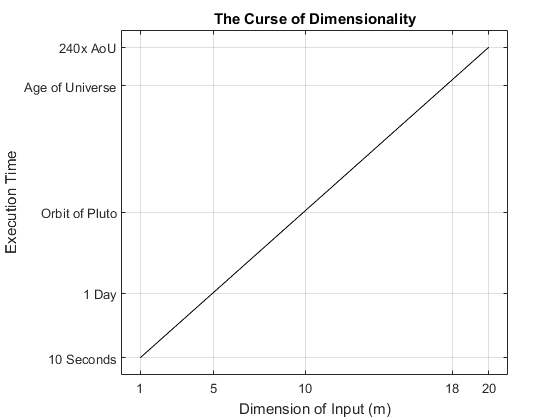
\includegraphics{../images/curse_of_dimensionality}
 \caption{The execution time of many studies increases exponentially with the dimensionality of parameter space.}
 \label{fig:dimensionality}
\end{wrapfigure}

This paragraph should introduce the Curse of Dimensionality; the motivation behind Dimension Reduction. Lorem ipsum dolor sit amet, consectetur adipiscing elit. Mauris eu vehicula diam, quis tempus nunc. Nunc rutrum leo vitae placerat lacinia. Nulla sodales, sem quis imperdiet dictum, felis ante iaculis erat, vel tincidunt odio urna eget erat. Sed eu faucibus neque, tempus porttitor augue. Fusce nec semper lectus, a varius est. Fusce ultricies euismod enim vel porta. Suspendisse accumsan, libero dignissim consectetur eleifend, nulla ligula dictum tellus, sit amet placerat risus diam in ipsum. Donec leo turpis, porta sit amet ipsum sit amet, mattis varius ipsum. Praesent ac ante aliquet, lacinia nulla in, interdum nunc. Curabitur dictum porta ipsum, at egestas libero blandit vitae. Sed tristique viverra erat. Ut mauris eros, bibendum sed massa vel, congue dignissim tortor. Interdum et malesuada fames ac ante ipsum primis in faucibus. Nullam consectetur sed sapien sed sollicitudin. Curabitur et justo a dolor pulvinar tincidunt non ac lacus. 

\begin{wrapfigure}{L}{0.5\linewidth}
 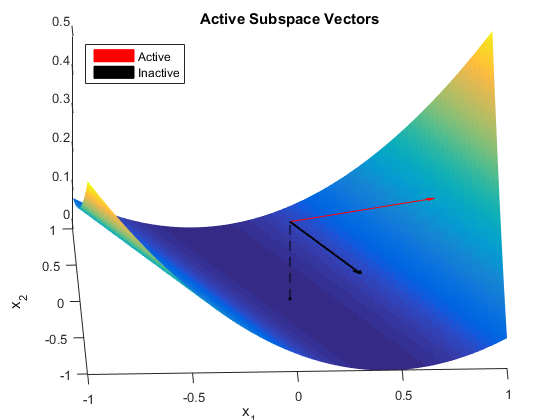
\includegraphics{../images/surface_plot}
 \caption{Example of Active Subspaces.}
 \label{fig:as_example}
\end{wrapfigure}

This paragraph should introduce Active Subspaces, give an example of its use, and discuss some limitations. \cite{constantine2015} Lorem ipsum dolor sit amet, consectetur adipiscing elit. Mauris eu vehicula diam, quis tempus nunc. Nunc rutrum leo vitae placerat lacinia. Nulla sodales, sem quis imperdiet dictum, felis ante iaculis erat, vel tincidunt odio urna eget erat. Sed eu faucibus neque, tempus porttitor augue. Fusce nec semper lectus, a varius est. Fusce ultricies euismod enim vel porta. Suspendisse accumsan, libero dignissim consectetur eleifend, nulla ligula dictum tellus, sit amet placerat risus diam in ipsum. Donec leo turpis, porta sit amet ipsum sit amet, mattis varius ipsum. Praesent ac ante aliquet, lacinia nulla in, interdum nunc. Curabitur dictum porta ipsum, at egestas libero blandit vitae. Sed tristique viverra erat. Ut mauris eros, bibendum sed massa vel, congue dignissim tortor. Interdum et malesuada fames ac ante ipsum primis in faucibus. Nullam consectetur sed sapien sed sollicitudin. Curabitur et justo a dolor pulvinar tincidunt non ac lacus.

This paragraph should briefly introduce the idea of Active Manifolds.

\section{Seeking Active Manifolds}

\begin{equation}
  \label{eq:inactive_manifold}
  \mW(\vx)^T \nabla f(\vx) = 0
\end{equation}%
\nomenclature{$\vx$}{Input vector}%
\nomenclature{$f(\vx)$}{Scalar quantity of interest}%
\nomenclature{$\nabla f(\vx)$}{Gradient of QoI}%
\nomenclature{$\mW(\vx)$}{Manifold vector}%

\section{Conclusion}

This had been a brief example of some of the more advanced options
available for \LaTeX.
Please see the documentation for each package for extended discussion or
usage.

% produces the bibliography section when processed by BibTeX
\bibliography{bibtex_database}
\bibliographystyle{aiaa}

\end{document}

% - Release $Name:  $ -
